\documentclass[11pt]{article}
\usepackage{icmlko}
\begin{document}

\title{옆방에도 못 건너간다 --- 같은 플랫폼 · 같은 자 · 같은 해, 나라만 다른 도메인}
\author{월드모델 실험실}
\date{노트 398 · 2026년 8월 2일}
\maketitle

\begin{abstract}
노트 397이 안 본 도메인(비게임 앱)에서 전이 $\approx 0$ 을 보고, 한계를
크게 적었다 --- \emph{비게임 앱은 IP 출시가 아니라서 의도한 범위보다
어려운 시험일 수 있다.} 그 도피로를 막는 시험을 찾았다.

\textbf{이미 갖고 있었다.} \texttt{manga\_axes} 는 국가 필터로 JP 만
남긴다. 그래서 AniList \textbf{한국 만화 1,716행이 한 번도 학습에 안
들어갔다.} 같은 플랫폼 · 같은 라벨(서재 등록 수) · 같은 매체 · 같은 축
코드 --- \textbf{나라만 다르다.}

2025년 이후 유보에서 재면 라벨 퍼짐이 $0.266$ 대 $0.264$(비 1.01), 중앙이
$3.096$ 대 $3.054$ 로 \textbf{짝이 저절로 맞는다.}

\begin{center}
\begin{tabular}{lrrrr}
\hline
 & 행 & 라벨 SD & 모형 $\rho$ & 편상관(날짜 통제) \\
\hline
JP 만화 (\textbf{학습에 든 도메인}) & 258 & 0.264 & $+0.3250$ & $\mathbf{+0.3196}$ \\
KR 만화 (\textbf{한 번도 안 본 도메인}) & 322 & 0.266 & $-0.1220$ & $\mathbf{-0.1261}$ \\
\hline
\end{tabular}
\end{center}

\textbf{$+0.32$ 에서 $-0.13$ 이다.} 전이가 약한 게 아니라 \textbf{음수}다.

그리고 거리로 줄이 안 선다 --- 먼 도메인(비게임 앱)이 $+0.08$ 인데
가까운 도메인(KR 만화)이 $-0.13$ 이다. \textbf{``앱은 너무 멀었다''는
설명이 여기서 죽는다.} 가르는 것은 거리가 아니라 \emph{그 행들이 학습에
들었나}다.

\textbf{다른 것은 하나뿐이다.} 플랫폼 · 라벨 자 · 매체 · 시기 · 라벨 퍼짐 ·
라벨 중앙 · 축 · 모형이 전부 같고, \textbf{그 나라 행이 학습에 들었는지만
다르다.}
\end{abstract}

\section{왜 이 짝이 좋은가}

노트 397의 약점은 도메인이 하나이고 그 하나가 유틸리티 앱이었다는 것이다.
공유 축 다섯(타깃 폭 · 장소 격 · 진입 마찰 · 매체 밀기 · 굿즈 규모)이
가계부 앱에서 무슨 뜻인지 애매하니, 전이가 0 인 것이 \emph{모형이 못
건너가서}인지 \emph{축이 그 도메인에서 무의미해서}인지 갈리지 않았다.

KR 만화는 그 애매함이 없다. 축이 재는 것이 화수 · 권수 · 태그 수 · 작가
수인데 한국 만화에서도 똑같은 뜻이다. 라벨도 같은 사이트의 같은 계수기다.
\textbf{축과 라벨이 뜻을 유지하는 채로 학습 여부만 바뀌는 짝}이라
노트 397이 못 가른 것을 가른다.

\begin{figure}[t]
\centering
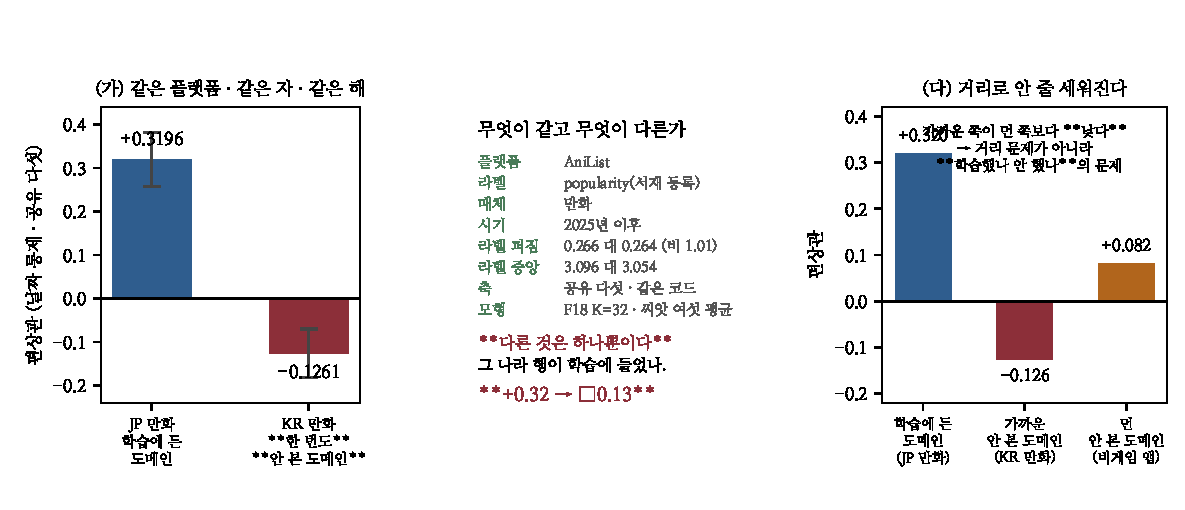
\includegraphics[width=\linewidth]{figs/fig398.pdf}
\caption{\textbf{(가)} 짝 맞춘 두 무리. 막대는 $1/\sqrt{n}$.
\textbf{(나)} 여덟 가지가 같고 하나만 다르다. \textbf{(다)} 거리로 줄이
안 선다 --- 가까운 쪽이 먼 쪽보다 낮다.}
\label{fig:main}
\end{figure}

\section{쟀다}

\texttt{manga\_axes} 의 국가 필터를 KR 로 돌려 축을 만들었다(코드는 한 줄도
안 고쳤다 --- 상수만 바꿨다). 챔피언 F18($K{=}32$)을 \textbf{열한 도메인
학습 행으로만} 적합하고, 두 무리를 같은 절차로 쟀다:

\begin{itemize}
\item \textbf{공유 축 다섯만} --- KR 은 트렌드 · 위키가 없으므로 JP 도
못 쓰게 막는다(노트 397의 대조).
\item \textbf{날짜 통제 편상관} --- 라벨이 누적이라 날짜가 섞인다.
\item \textbf{씨앗 여섯 순위 평균} --- 노트 395.
\item \textbf{2025년 이후 유보만} --- JP 쪽이 학습에 안 든 행이어야 한다.
\end{itemize}

\textbf{퍼짐을 맞추려고 아무것도 안 했는데 맞았다.} KR 0.266 · JP 0.264
(비 1.01), 중앙 3.096 · 3.054, 범위 $2.80\sim4.12$ · $2.80\sim4.35$.
노트 376 이후 퍼짐 대조를 손으로 만들어 왔는데 이번에는 자연히 짝이다.

\section{읽는 법}

\textbf{첫째, 전이가 음수다.} $-0.1261 \pm 0.056$ 이라 0 과도 구별된다.
모형이 KR 만화에서 \emph{거꾸로} 줄을 세운다. 노트 372가 만화 KR 을
$-0.16$ 으로 쟀던 것이 다른 절차에서 재현됐다.

\textbf{둘째, 거리가 설명이 아니다.} 노트 397의 앱은 훨씬 먼 도메인인데
$+0.08$ 이고 KR 만화는 옆방인데 $-0.13$ 이다. 거리로 정렬되지 않으므로
``더 가까운 도메인을 고르면 된다''는 길이 막힌다.

\textbf{셋째, 무엇이 남았나.} 도메인 원핫이다. F18 은 도메인마다 원핫을
하나씩 갖고, 모르는 도메인에는 전부 0 을 준다. 그러면 예측이 \emph{공유
계수}만으로 나오는데, 그 공유 계수가 열한 도메인의 평균이라 어느 한
도메인에도 잘 안 맞는 것으로 읽는다. \textbf{다만 이것은 관측이 아니라
설명이라 다음 노트로 넘긴다} --- 원핫을 켜고 껐을 때의 차를 재면 갈린다.

\section{그래서 판을 어떻게 읽나}

\textbf{판 0.4476 은 ``열한 도메인 안에서''의 수다.} 그 밖으로 나가면
$+0.08$(먼 도메인) 또는 $-0.13$(옆방)이다. 두 번 다 재 봤고 두 번 다
0 이하다.

\textbf{그러면 판정치의 이름을 고쳐야 한다.} 지금까지 대장에 ``판''이라고만
적어 왔는데, 이 수가 뜻하는 것은 \emph{학습에 든 도메인 안에서의 평균
순위 상관}이다. 대장과 노트에 \textbf{``판(학습 도메인 안)''} 으로 적는다.
IP 파운데이션이라는 목표는 그 밖을 주장하는 것이고, \textbf{그 주장은 지금
증거가 없다.}

\textbf{안 바꾸는 것.} 관문은 그대로다 --- 두 팔을 같은 도메인 집합에서
짝지어 견주는 데는 이 문제가 안 생긴다. 이번 사이클의 채택들(펀딩 · 웹툰 ·
만화 · 애니 학습 확장, $K{=}32$)은 전부 그 틀 안이라 영향이 없다.

\section{남은 것}

\begin{center}
\begin{tabular}{lll}
\hline
항목 & 왜 값이 큰가 & 어떻게 \\
\hline
원핫이 범인인가 & 유일하게 남은 설명 & 원핫 끄고 학습해 KR 을 다시 잰다 \\
KR 을 넣으면 사나 & 넣으면 되는지가 실무 답 & KR 학습 추가 후 재측정 \\
세 번째 짝 & 둘로는 아직 얇다 & CN 만화 352행이 같은 자리에 있다 \\
판정치 이름 & 지금 이름이 과장한다 & 대장·노트 표기 바꾸기 \\
\hline
\end{tabular}
\end{center}

\end{document}
